\documentclass[a4paper]{report}

\pdfminorversion=5 
\pdfcompresslevel=9
\pdfobjcompresslevel=2

%====================== PACKAGES ======================

\usepackage[french]{babel}
\usepackage[utf8x]{inputenc}
\usepackage{titlesec}
\usepackage{pgfplots}
% \usepackage{subcaption}
%pour gérer les positionnement d'images
\usepackage{float}
\usepackage{amsmath}
\usepackage{amssymb}
\usepackage{graphicx}
\usepackage[colorinlistoftodos]{todonotes}
\usepackage{url}
%pour les informations sur un document compilé en PDF et les liens externes / internes
\usepackage{hyperref}
%pour la mise en page des tableaux
\usepackage{array}
\usepackage{tabularx}
%pour utiliser \floatbarrier
%\usepackage{placeins}
%\usepackage{floatrow}
%espacement entre les lignes
\usepackage{setspace}
%modifier la mise en page de l'abstract
\usepackage{abstract}
%police et mise en page (marges) du document
\usepackage[T1]{fontenc}
\usepackage[top=2cm, bottom=2cm, left=2cm, right=2cm]{geometry}
%Pour les galerie d'images
\usepackage{subfig}
\usepackage[shortlabels]{enumitem}
\usepackage[toc]{glossaries}
\usepackage{caption}
\usepackage{ragged2e}
\usepackage{listings}
\usepackage{color}
\usepackage{pgfplotstable}



\def\nbR{\ensuremath{\mathrm{I\! R}}}


\definecolor{dkgreen}{rgb}{0,0.6,0}
\definecolor{gray}{rgb}{0.5,0.5,0.5}
\definecolor{mauve}{rgb}{0.58,0,0.82}

\lstset{frame=tb,
  language=sql,
  aboveskip=3mm,
  belowskip=3mm,
  showstringspaces=false,
  columns=flexible,
  basicstyle={\small\ttfamily},
  numbers=none,
  numberstyle=\tiny\color{gray},
  keywordstyle=\color{blue},
  commentstyle=\color{dkgreen},
  stringstyle=\color{mauve},
  breaklines=true,
  breakatwhitespace=true,
  tabsize=3
}





\setcounter{tocdepth}{4}
\setcounter{secnumdepth}{4}

\makeglossaries

\titleformat{\chapter}[display]
  {\normalfont\bfseries}{}{0pt}{\Huge}


\begin{document}
%régler l'espacement entre les lignes
\newcommand{\HRule}{\rule{\linewidth}{0.5mm}}
\renewcommand{\abstractname}{Résumé }
\newcommand{\Csharp}{%
  {\settoheight{\dimen0}{C}C\kern-.05em \resizebox{!}{\dimen0}{\raisebox{\depth}{\#}}}}


%page de garde
\begin{titlepage}
    \begin{center}
    
    % Upper part of the page. The '~' is needed because only works if a paragraph has started.
    \includegraphics[width=0.7\textwidth]{images/esirem.png}~\\[1cm]
    
    \textsc{\LARGE Université de Bourgogne}\\[1.5cm]
    
    \textsc{\Large }\\[0.5cm]
    
    % Title
    \HRule \\[0.4cm]
    
    {
    \huge \bfseries Projet 4A - Prédiction de score en Formule 1\\[0.4cm]
    }
    
    \HRule \\[1.5cm]
    
    % Author and supervisor
    \begin{minipage}{0.4\textwidth}
    \begin{flushleft} \large
    \emph{Auteur :}\\
    Benjamin \textsc{MILHET} 

    \end{flushleft}
    \end{minipage}
    \begin{minipage}{0.4\textwidth}
    \begin{flushright} \large
    \emph{Professeur :} \\
    Mme. \textsc{ANSART}\\
    
    \end{flushright}
    \end{minipage}

   

    
    \vfill
        
    
\includegraphics[width=0.5\textwidth]{images/logoF1.jpg}~\\[3cm]
    % Bottom of the page
    \href{mailto:benjamin_milhet@etu.u-bourgogne.fr}{benjamin\_milhet@etu.u-bourgogne.fr}\\[.5cm]
    
    \end{center}
    \end{titlepage}

%page blanche
\newpage
~
%ne pas numéroter cette page
\thispagestyle{empty}
\newpage

\tableofcontents
\thispagestyle{empty}
\setcounter{page}{0}
\setcounter{page}{1}
%ne pas numéroter le sommaire

\newpage

%espacement entre les lignes d'un tableau
\renewcommand{\arraystretch}{1.5}

%====================== INCLUSION DES PARTIES ======================

%recommencer la numérotation des pages à "1"
\setcounter{page}{1}

\chapter{Introduction}

L'objectif de ce projet de 4e année est d'approfondir le machine learning introduit lors de ma formation à l'ESIREM et de pouvoir découvrir de nouveaux aspect d'un domaine très large et en pleine expansion. Dans ce projet, nous allons faire des recherches sur les différents types d'apprentissages et leurs algorithmes, puis nous allons choisir un dataset sur le site Kaggle permettant de réaliser le projet et nous allons déterminer son types d'apprentissage et tester différents algorithmes de machine learning adapté a ce sujet.\\

Dans ce projet, nous allons explorer différents algorithmes de Machine Learning pour prédire le nombre de points qu'un pilote de Formule 1 peut gagner lors d'un Grand-Prix. Nous allons utiliser des données de Formule 1 depuis 1950 pour entraîner nos modèles de prédiction. Nous allons utiliser différents algorithmes d'apprentissage automatique pour traiter les données, tels que la régression linéaire, la régression Lasso et la régression Ridge. Nous allons également utiliser des techniques de visualisation pour mieux comprendre les données et les résultats des modèles. Ce projet est une introduction pour découvrir les différents types d'apprentissage de Machine Learning avec un sujet que j'apprécie qui est la Formule 1.
\chapter{Découverte du machine learning}
\section{Quelle est la différence entre apprentissage supervisé et non-supervisé ?}
Un apprentissage supervisé possède des données en entrée et en sortie. Ce type d’apprentissage possède un training set, un ensemble de données qui permet d’entraîner notre algorithme avec des données en entre à tester et les différentes solutions associées. Cela lui permet d’avoir une base pour ensuite étudier de nouveaux individus et d’avoir une idée de quel type de solution l’algorithme doit chercher.\\

Pour l’apprentissage non supervisé, il n’y a pas de données en sortie mais juste en entrée. C’est à l’algorithme de déduire les points importants et de proposer ses solutions sans avoir été entraîné auparavant.

\section{Quelle est la différence entre classification et régression ? Est-ce de l’apprentissage supervisé ou non-supervisé ?}
La classification et la régression sont 2 types d’algorithmes utilisant un apprentissage supervisé. On utilise la classification lorsque les solutions souhaitées sont des catégories comme des pommes ou des oranges. Alors que la régression est utilisée pour des valeurs numériques comme pour prédire le chiffre d’affaires d’une entreprise. La régression essaye de comprendre les relations entre les différentes variables.


\section{Qu’est-ce que du clustering ? Quelle est la différence avec la classification ?}
La principale différence entre la classification et le clustering est que la classification utilise un apprentissage supervisé alors que le clustering suit un apprentissage non supervisé. Le clustering se base sur les similitudes des paires en entrée, et sur son expérience au fur et à mesure de tester différentes entrées. Le temps d’exécution peut être très élevé si le nombre d’exemples en entrée est très élevé (plusieurs millions)

\newpage
\section{Sur kaggle ou driven-data, choisissez 5 exemples de compétitions et dites quel est le type de problème (classification, régression, clustering ou autre)}

\href{https://www.kaggle.com/competitions}{Liste des compétitions sur Kaggle}


\subsection{Compétition 1} 
\href{https://www.kaggle.com/competitions/house-prices-advanced-regression-techniques/data}{Compétition 1 sur la prédiction du prix d'une maison}\\

On remarque que le jeu de donnée possède un jeu de données d’entraînement et un jeu de données à tester. On est donc sur un apprentissage supervisé. Il faut trouver une valeur numérique pour prédire le prix de vente. Je pense qu’il faut utiliser une régression.


\subsection{Compétition 2} 
\href{https://www.kaggle.com/competitions/spaceship-titanic/overview}{Compétition 2 sur la prédiction de quel passager seront transportés dans une autre dimension}\\

On remarque que le jeu de donnée possède un jeu de données d’entraînement et un jeu de données à tester. On est donc sur un apprentissage supervisé. Il faut prédire si le passager va voyager dans une autre dimension ou non. Je pense qu’il faut utiliser une classification parce que c’est un choix binaire.


\subsection{Compétition 3} 
\href{https://www.kaggle.com/competitions/titanic/overview}{Compétition 3 sur la prédiction des survivants du Titanic}\\

On remarque que le jeu de données possède un jeu de données d’entraînement et un jeu de données à tester. On est donc sur un apprentissage supervisé. Il faut prédire si le passager du Titanic va mourir ou non. Je pense qu’il faut utiliser une classification parce que c’est un choix binaire.


\subsection{Compétition 4} 
\href{https://www.kaggle.com/competitions/nlp-getting-started}{Compétition 4 sur la prédiction de si le contenu d'un tweet est réel ou non}\\

On remarque que le jeu de donnée possède un jeu de données d’entraînement et un jeu de données à tester. On est donc sur un apprentissage supervisé. Il faut prédire si l’information dans le tweet est vraie ou non. Je pense qu’il faut utiliser une classification parce que c’est un choix binaire.


\subsection{Compétition 5} 
\href{https://www.drivendata.org/competitions/66/flu-shot-learning/page/211/}{Compétition 5 sur la prédiction de quel personne vont recevoir leusr doses de vaccin}\\

On remarque que le jeu de donnée possède un jeu de données d’entraînement et un jeu de données à tester. On est donc sur un apprentissage supervisé. Il faut prédire si n individu va se faire vacciner pour h1n1 ou/et pour la grippe saisonnière ou non. Je pense qu’il faut utiliser une classification parce que c’est un choix binaire, il faut classer les personnes en fonction de quel vaccin ils vont choisir ou non.


\section{Quel type de problème de machine learning vous semble le plus répandu ?}
Je remarque déjà que le type d’apprentissage le plus utilisé est l’apprentissage supervisé. On en déduit donc 2 types de problèmes qui sont le plus répandus et qui sont la classification et la régression. D’après les exemples précédents, j’ai l’impression que le problème de machine learning le plus répandu est la classification.
\chapter{Choix du sujet}

\section{Découverte de Kaggle}
Pour ce projet, je devais choisir suje, un domaine sur lequel je devais utiliser des algorithmes d'inteligences artificielles. Je me suis donc rendu sur le site Kaggle qui comprend des competitions et des dataset. Un dataset est un ensemble de données sur un sujet. Ce site comprend aussi des formations pour prendre en main python et ses bibliothèques pour le traitement des données comme Numpy ou Scikit-Learn. Avant de choisir un dataset pour ce projet, j'ai commencé par effectuer la formation "Python" et "Intro to Machine Learning" qui m'a permis de mieux comprendre l'utilisation de Scikit-Learn.

\section{Pourquoi ce domaine ?}
Une fois une petite base acquise, je me suis rendu sur la catégorie dataset de Kaggle pour voir l'ensemble des datasets disponibles. C'est en faisant mes recherches que je suis tombé sur un dataset contenant des données sur les différents championnats de Formule 1 depuis 1950. La formule 1 est un sport que je suis depuis plus de 10 ans grâce à mon père qui m'a transmis sa passion. Après avoir regarder son contenu et trouver un objectif avec celle-ci, j'ai fait valider mon sujet par Mme. Ansart, ma tutrice du projet, pour pouvoir continuer mon projet avec ce dataset.

\section{Explication de la Formule 1}
Un championnat de Formule 1 est une série de courses automobiles qui se déroulent sur un ensemble de course à travers le monde. Les équipes de F1 sont composées de constructeurs automobiles et de pilotes professionnels qui concourent pour le titre de champion du monde de F1. Les courses se déroulent sur une saison qui dure généralement de mars à décembre, avec des courses chaque week-end. Les pilotes sont classés en fonction de leur performance lors de chaque course, et le pilote ou l'équipe avec le plus de points à la fin de la saison est déclaré champion.\\

Un Grand Prix de Formule 1 est une course qui fait partie de ce championnat. Les Grand Prix se déroulent sur des circuits de course spécialement conçus et sont généralement assez longs, avec des longueurs allant de 5 à 7 kilomètres. Avant chaque Grand Prix, il y a des séances d'essais libres et de qualifications pour permettre aux pilotes de se familiariser avec le circuit et de déterminer leur place de départ sur la grille. Les qualifications consistent en plusieurs tours rapides pour déterminer la position de départ des pilotes, avec les meilleurs temps qui obtiennent les positions les plus avancées sur la grille de départ. La course elle-même dure au maximum 2 heures, avec les pilotes qui effectuent un certain nombre de tours du circuit. Les pilotes s'arrêtent pour changer de pneus pendant la course, ce qui peut influencer leur stratégie et leur performance. Seul les dix premiers d'une course gagnent des points allant de 25 à 1 points pour le 10e.


\newpage
\section{Le Dataset}

\href{https://www.kaggle.com/datasets/thedevastator/formula-one-racing-a-comprehensive-data-analysis}{Dataset sur la formule 1 utilisée pour la suite du projet}\\

\subsection{Explication du contenu du dataset}

\subsubsection{Fichier Circuits.csv}
Le fichier Circuits.csv contient l'ensemble des circuit de Formule 1 avec leurs noms, leurs pays et leurs positions géographiques.

\subsubsection{Fichier Constructors.csv}
Le fichier Constructors.csv contient l'ensemble des écuries de Formule 1 qui ont éxister. Ce fichier liste uniquement le nom des écuries et leurs nationalités. Une écurie de F1 est composé de deux pilotes principaux, de pilote réserviste et de nombreux ingénieurs pour concevoir la voiture et réaliser des stratégies pour les différentes courses.

\subsubsection{Fichier Drivers.csv}
Le fichier Drivers.csv comprend l'ensemble des pilotes qui ont au moins participés à un grand prix de F1. Ce dataset contient aussi le nom, le prénom et la date de naissance de chacun des pilotes.

\subsubsection{Fichier Lap\_times.csv}
Le fichier Lap\_times.csv contient le temps et la position de chaque tours de chaque pilote pour chacun des Grand-prix qu'ils ont effectuées. Nous avons à notre disposition le temps en Minute/Seconde/Milliseconde et le temps en Milliseconde ainsi que sa position pour le tour.

\subsubsection{Fichier Pit\_stops.csv}
Le fichier Pit\_stops.csv contient tous les arrêts au stand avec à quelle moment de la course un pilote effectue cet arret, à quelle tour et la durée de l'arrêt au stand. Durant un Grand-prix, chaque pilote doit au moins effectuer un arrêt au stand pour mettre un autre type de pneux.

\subsubsection{Fichier Qualifying.csv}
Le fichier Qualifying.csv comprend la position du pilote après la séance de classification et ses 3 meilleurs temps des 3 séances de qualifications. Les qualifications se divisent en 3 parties appelée Q1, Q2 et Q3. Après la première seance de qualification Q1, seulement les 15 meilleurs pilotes accèdent à la Q2 et seulement les 10 meilleurs de la séance Q2 accèdent à la dernière seance de qualification Q3 qui déterminira le palcement finale sur la grille de départ.

\subsubsection{Fichier Results.csv}
Le fichier Results.csv contient l'ensemble des résultats de chacun des pilotes pour chaque course q'ils ont effectuées avec leur position, leur nombre de point gagner et leur position de départ. C'est un des fichiers les plus importants parce que c'est celui qui contient le nombre de points gagner par course pour chaque pilote et avec son écuries associées.

\subsubsection{Fichier Races.csv}
Le fichier Races.csv contient l'ensemble des grand-prix réalisé depuis 1950 et avec leur date, l'heure et la ville ou se situe le circuit.

\subsubsection{Fichier Constructor\_standings.csv}
Le fichier Constructor\_standings.csv contient le nombre de points et la position au classement de chacune des écuries de Formule 1 pour chaque championnat mondial annuel.

\newpage

\subsection{Visualisation des données}









\chapter{Choix du type d'algorithme}
Ce dataset contient des informations sur l'ensemble des courses de Formule 1 depuis l'année 1950. Il y a plusieurs fichiers des datas sur les pilotes, les tracées des courses, sur les écuries, et l'ensemble des résultats pour les qualifications, course sprint et (vraie) course. Le fichier le plus important est Result.csv car il contient les résultats de chaque course avec le score de chaque pilote et le lieu. L'objectif est de trouver un modèle qui permet de prédire le nombre de points qu'un pilote gagne à la fin d'un grand-prix. Pour cela, nous devons trouver les variables qui ont le plus d'impact sur le nombre de points d´un pilote. Il s'agit d'un apprentissage supervisé car nous avons un jeu de données d'entraînement et un jeu de données à tester. Nous devons prédire un nombre de point d'un pilote à la fin d'une course. De plus, il nous faudra utiliser une régression parce que nous devons déterminer une valeur numérique. Finalement, il ne me restait plus que à savoir comment choisir mes données. Pour cela, deux possibilités s'offrait à moi, utiliser l'ensemble des données disponibles pour déterminer le nombre de points que va gagner un pilote pour une course, ou utiliser les données du pilote sur le quelle je vais effectuer des prédictions. J'ai choisi la 2e options parce que chaque pilote possède une façon unique de piloter avec leurs réflexes et leurs différentes limites.


\section{Algorithme 1 : Algorithme de régression linéaire simple}
J'ai commencé par analyser mes données et sélectionner celle qui me semble importante pour commencer. En premiers lieux j'ai commencé par une régression linéaire simple pour prendre en main les différentes bibliothèques. J'ai pris comme paramètre le nombre de points d'un pilote par rapport à ses différentes courses. Les résultats ne sont pas très concluants pour plusieurs raisons. La première est que la courbe de prédiction et suit une loi y = ax + b. La seconde raison est que le nombre de points gagnés par un pilote sur une course ne dépend pas uniquement de sa position de départ, mais de beaucoup plus de facteur cité dans le chapitre consacré au Dataset.

\begin{figure}[H]
    \centering
    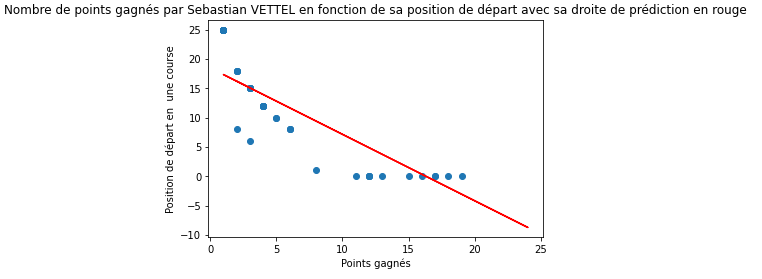
\includegraphics[width=.8\textwidth]{images/RegVettel.png} 
    \caption{Régression linéaire simple du nombre de point gagner par rapport à sa position de départ du pilote S. Vettel}
\end{figure}

\section{Algorithme 2 : Algorithmes de régression logistique}
Durant mes recherches, j'ai découvert la régression logistique, cependant, après des premières recherches, elle ne semble pas correspondre à mon problème. En effet, celle-ci est principalement utilisée pour une classification binaire. Notre problème est de déterminer le nombre de points gagner et cela n'est pas un choix entre deux solutions prédéfinies.

\newpage
\section{Choix d'un meilleur algorithme}

\href{https://scikit-learn.org/stable/tutorial/machine_learning_map/index.html}{Cheat-Sheet de Sckit-Learn}\\

\begin{figure}[H]
    \centering
    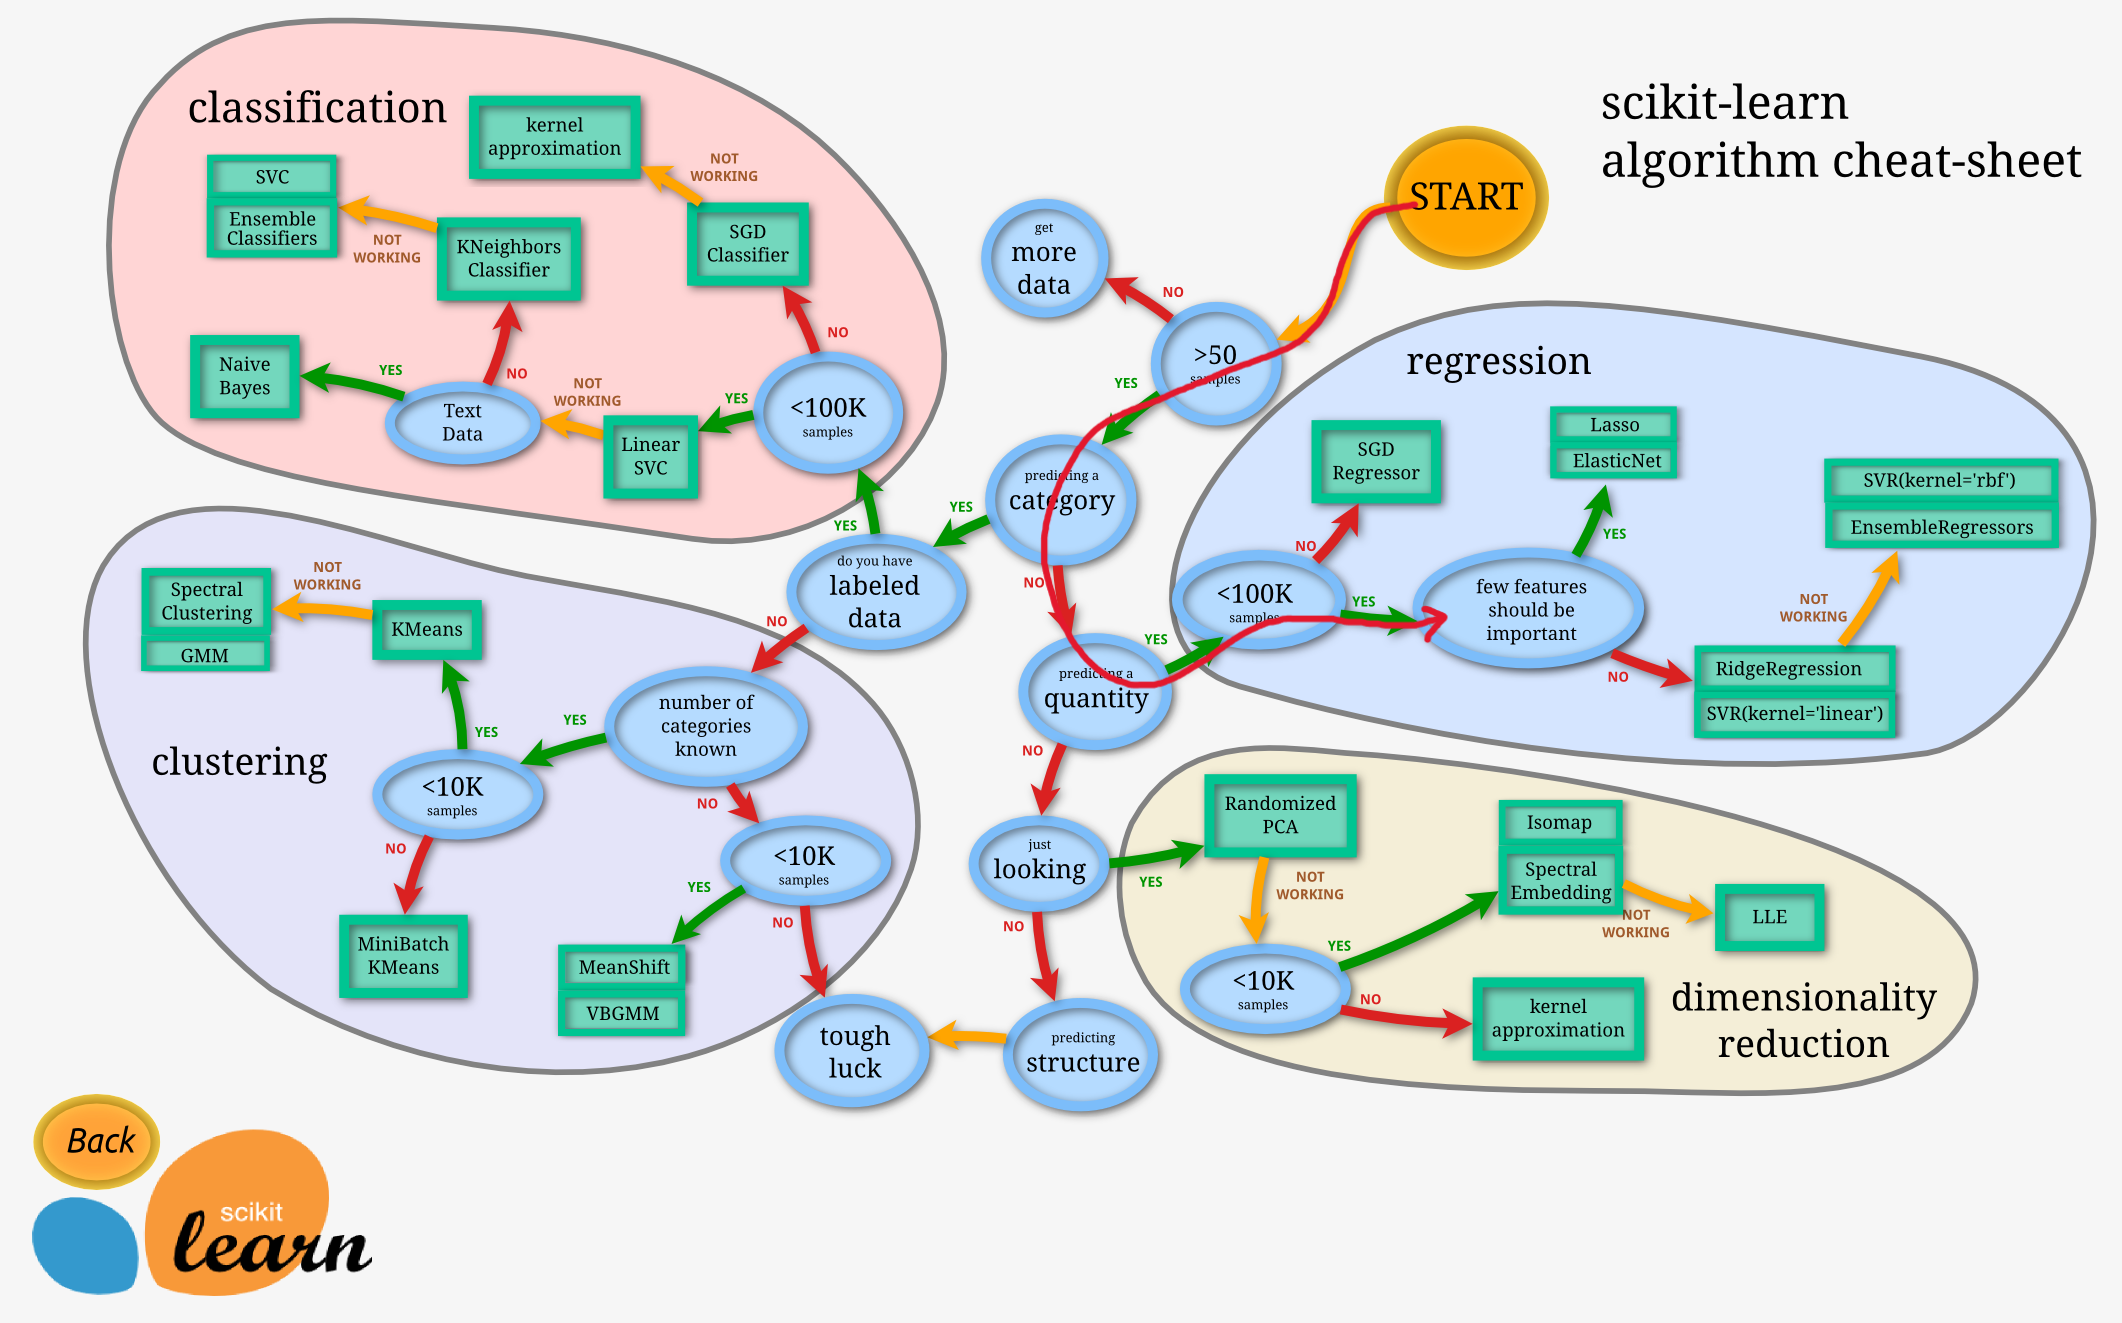
\includegraphics[width=1\textwidth]{images/cheat-sheet.png} 
    \caption{Chemin choisit pour mon projet sur la Cheat-Sheet}
\end{figure}
Étant données qu'aucun des premiers algorithmes était intéressants au vu des résultats à cause principalement du fait qu'il ne prend qu'un seul paramètre en entrée. Je me suis donc dirigée vers la cheat-sheet de scikit-learn qui nous permet de déterminer quel algorithme utiliser pour tenter d'atteindre notre objectif de prédiction. Nous avons déjà plus de 50 exemples et ne nous cherchons pas à prédire une catégorie. Ensuite nous voulons prédire une quantité et nous avons moins de 100 000 exemples, ce qui mène au dernier choix qui nous demande si peu de caractéristiques devraient être importantes ou non. Nous cherchons donc à réaliser une régression et pour ce dernier choix, je vais faire des tests avec les différents algorithmes proposés pour chacun d'eux avec l'algorithme Lasso et la RidgeRegression. En effet ces deux algorithmes permettent de prendre plusieurs paramètres en entier afin que le résultat en sortit soit plus réaliste. Dans un Grand-prix de F1, ce n'est pas seulement sa position de dé part ou juste l'équipe à laquelle appartient un pilote, qui permet de savoir le nombre de points que va obtenir un pilote à la fin de la course, mais plutôt un ensemble de facteurs combinés. 

\section{Algorithme de régression LASSO}

Le premier algorithme de régression prenant plusieurs paramètres en entrée que je vais étudier est un algorithme de régression LASSO pour Least Absolute Shrinkage and Selection Operator et qui me permet de choisir les paramètres les plus importants dans l'ensemble de mes fichiers. En effet, pour prédire le nombre de points qu'un pilote de Formule 1 peut gagner, cet algorithme permet de sélectionner automatiquement les variables les plus importantes pour la prédiction. Dans le cas de la Formule 1, il y a souvent beaucoup de variables qui peuvent influencer les performances d'un pilote, telles que l'âge, l'expérience, la vitesse moyenne, les positions de départ en pole position, et l'ensemble des points déjà gagner par grand-prix. Le fait d'utiliser une régression Lasso pour sélectionner les paramètres les plus intéressants pourrait améliorer la précision des prédictions et éviter le sur-apprentissage.

\begin{figure}[H]
    \centering
    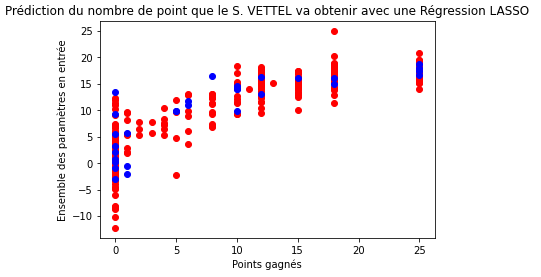
\includegraphics[width=.8\textwidth]{images/LASSOVettel.png} 
    \caption{Régression LASSO sur les données du pilote S. VETTEL}
\end{figure}

On observe en rouge les résultats obtenus avec le jeu d'entraînement et en bleu les résultats obtenus avec le jeu de test. Visuellement, les prédictions obtenues en bleu concordent avec les résultats du jeu d'entraînement. De plus, nous avons un Mean MAE de 4.073 (0.563), le score est faible ce qui indique un taux d'erreur acceptable mais que l'on peut toujours améliorer avec un algorithme ou en choisissant/remplaçant des données.



\chapter{Analyse des résultats}
\chapter{Difficultés rencontrées}
Ma principale difficulté rencontrée durant ce projet, mais aussi à travers l'ensemble de ce semestre est la sous-estimation du travail demandées dans certaine matière et la mauvaise gestion de mon temps libre pour mener à bien le projet de 4A. En effet, lors de la réalisation de ma première planification, je ne pensais pas avoir une charge de travail à la maison aussi importante pour la rédaction des différents rapports et la préparation aux partiels.\\ 

Une autre difficulté au début du projet était ma faible connaissance du langage Python et de ses librairies pour le Machine Learning. 

\chapter{Points à améliorer}


\chapter{Conclusion}
\chapter{Bibliographie}

\section{Sites Internet}

 - \href{https://www.ibm.com/cloud/blog/supervised-vs-unsupervised-learning}{Supervised vs. Unsupervised Learning: What’s the Difference? - IBM}\\

 - \href{https://developers.google.com/machine-learning/clustering/clustering-algorithms?hl=en}{Clustering Algorithms - Google}\\

 - \href{https://www.kaggle.com/competitions}{Kaggle}\\

 - \href{https://www.kaggle.com/learn}{Kaggle Learn}\\

 - \href{https://scikit-learn.org/stable/index.html}{Scikit-Learn}\\

 - \href{https://scikit-learn.org/stable/tutorial/machine_learning_map/index.html}{Cheat-Sheet de Sckit-Learn}


\section{Livre}
 - \href{https://www.oreilly.com/library/view/le-machine-learning/9782412034460/}{Le Machine Learning avec Python de Andreas C. MÜLLER et Sarah GUIDO}

\section{Vidéos}

 - \href{https://www.youtube.com/watch?v=YfAgP-xKi30&list=LL&index=2}{Tout savoir sur la régression pénalisée (Ridge/Lasso/ElasticNet) - LES MODELES LINEAIRES \#9 }\\

 - \href{https://www.youtube.com/watch?v=WLmOFlSxYTY&list=LL&index=25}{ Coder régression linéaire Simple - Exemple Pratique - Machine Learning / Apprentissage automatique }




\end{document}
